\documentclass{article}

\usepackage{amsmath, amsthm, amssymb, amsfonts}
\usepackage{thmtools}
\usepackage{graphicx}
\usepackage{setspace}
\usepackage{geometry}
\usepackage{float}
\usepackage{hyperref}
\usepackage[utf8]{inputenc}
\usepackage[english]{babel}
\usepackage{framed}
\usepackage[dvipsnames]{xcolor}
\usepackage{tcolorbox}

\colorlet{LightGray}{White!90!Periwinkle}
\colorlet{LightOrange}{Orange!15}
\colorlet{LightGreen}{Green!15}

\newcommand{\HRule}[1]{\rule{\linewidth}{#1}}

\declaretheoremstyle[name=Theorem,]{thmsty}
\declaretheorem[style=thmsty,numberwithin=section]{theorem}
\tcolorboxenvironment{theorem}{colback=LightGray}

\declaretheoremstyle[name=Proposition,]{prosty}
\declaretheorem[style=prosty,numberlike=theorem]{proposition}
\tcolorboxenvironment{proposition}{colback=LightOrange}

\declaretheoremstyle[name=Principle,]{prcpsty}
\declaretheorem[style=prcpsty,numberlike=theorem]{principle}
\tcolorboxenvironment{principle}{colback=LightGreen}

\setstretch{1.2}
\geometry{
    textheight=9in,
    textwidth=5.5in,
    top=1in,
    headheight=12pt,
    headsep=25pt,
    footskip=30pt
}

% ------------------------------------------------------------------------------

\begin{document}

% ------------------------------------------------------------------------------
% Cover Page and ToC
% ------------------------------------------------------------------------------

\title{ \normalsize \textsc{}
		\\ [2.0cm]
		\HRule{1.5pt} \\
		\huge \textbf{CoasterDex
		\HRule{2.0pt} \\ [0.6cm] \Large{software for detection and recognition of beer-coasters from images} \vspace*{10\baselineskip}}
		}
\date{}
\author{\textbf{Authors} \\ 
		David Pažout \& Dagur Elinór Kristinnson\\
		RU \\
		19.12.2023}

\maketitle
\newpage

\tableofcontents

\hspace{20pt}

\begin{abstract}
CoasterDex is a software for detection and classification of beercoasters in images and video.
It combines fine tuned Yolov5 based CNN with 
custom SIFT based instance level recognition algorithm 
to achieve high accuracy detection of beercoasters across varied environments.
\end{abstract}

\newpage

\section{Introduction}
% - problem statement & project idea. 
% - Relevant prior work reported by others.  Existing methods, software, and data sets that could be applied to your solution. 
% - How does your application, application area, or approach differ from the prior work?
\subsection{Problem Definition}
This problem is inspired by my friend who collects beercoasters. 
They have a collection of more then 200 unique beercoasters. 
Every time I'm in a pub and see a beercoaster I don't know if they already have it or not.
They aren't always available to be asked or they sometimes don't remember and bringing them a duplicate coaster is suboptimal.

Formal definition is as follows, we have a collection $C=\{c_1,...c_n | c_i \neq c_j;\ \forall i,j;\ i \neq j\}$ of images of unique beercoasters or coaster-scans from frontal view.
Given an input image $img$, the goal is to find all beercoasters $B=\{b_1...b_m\}$ present in the image 
and determine if a beercoaster $b \in B$ is also present in $C$. 
If $b$ isn't present in the collection we should add it to the collection ($C \leftarrow C \cup b$).

\subsection{Relevant Work}
We found a few papers tackling a similar or adjacent problems.
The oldest is a paper from 2011 solving postage stamp recognition from photo-scans \cite{}.
Since the paper was written before wide adoption of CNN it mainly uses custom, hand-crafted features and basic template matching for classification of relatively small number of stamps.
The authors in HotSpotter \cite{} try to match individual animals (not species) with past photos in a larger database with multiple instances of each individual.
In \cite{} CNN is used to tackle grocery product recognition. The authors approach the problem as classification of images into 100 plus classes.

Most of the approaches for the instance recognition were taken from two throughout overviews on the subject \cite{} \cite{},
where authors compare older SIFT based and newer CNN based approaches to this problem.

Working with small datasets can be tricky since it can lead to overfitted models. Using smaller models increases performance in these cases.\cite{} Data augmentation is also a powerful tool for these situations due to its ability to 
increase dataset size artificially. The technique revolves around creating artificial copies of images with slight variations in specific image attributes, brightness for example. Data augmentation does not alter any biases of the original data set which needs to be complete in its content. Augmenting can also be a lot of work, figuring out the extensiveness of the augmentation approach needs to be done iteratively. \cite{}

% add Finder background materials 

Majority of the previous approaches work with a static databases, e.g. the whole pipeline/algorithm have to be retrained if we wand to introduce a new type of sample.
They often have multiple scans/instances available for retrieval and aren't limited by the time it takes to detect and retrieve the relevant object.
We have only single instance of the coaster available in the collection and want to use our system in real-time environment where prolonged waiting times are inconvenient.
System also should easily scale to larger collections (thousands of items).

\section{Materials and Methods}
% - Methods, software, and datasets that you tested and selected. 
% - How did you adapt the methods for use in your application?
We decomposed the problem to two main parts: Finder and Matcher.
Finder is an image classification and localization algorithm and its goal is to find all
occurrences of beercoasters $B=\{b_1...b_m\}$ in the image $img$ with their appropriate bounding boxes.
Matcher is an instance level recognition/retrieval algorithm and its goal is to match 
a beercoaster from the collection $c \in C$ with a beercoaster $b$ present in the image $img$
or to determine that there is no matching beercoaster present in the image.

\subsection{Finder - Coaster Detection}

To implement a coaster finding program the utilized method was yolov5 object detection model small version. The model was fine tuned
with a custom dataset specifically designed to train coaster detection. Roboflow was used to label the dataset and perform augmentations.
With a functional coaster detection model, opencv was used to extract the given bounding boxes and then returned to the matcher for 
integration.

\subsection{Matcher - Instance Recognition}

There are many approaches to instance recognition/retrieval. 
The two most popular are "classic" SIFT based approaches and "modern" CCN based approaches.
The goal of both is to extract one (or multiple) feature vectors of fixed length from the image and compare them to feature vector(s) extracted from the images in the collection and retrieve the most similar images based on similarity of those feature vectors.
The general pipeline is summarized in fig1.
It consist of three steps: feature extractions, encoding and indexing/search.
We opted for a compact representation of the final encoded feature vector, this enables us to easily test both SIFT and CNN base approaches with Nearest Neighbor (NN) search.

\begin{figure}[H]
    \center
    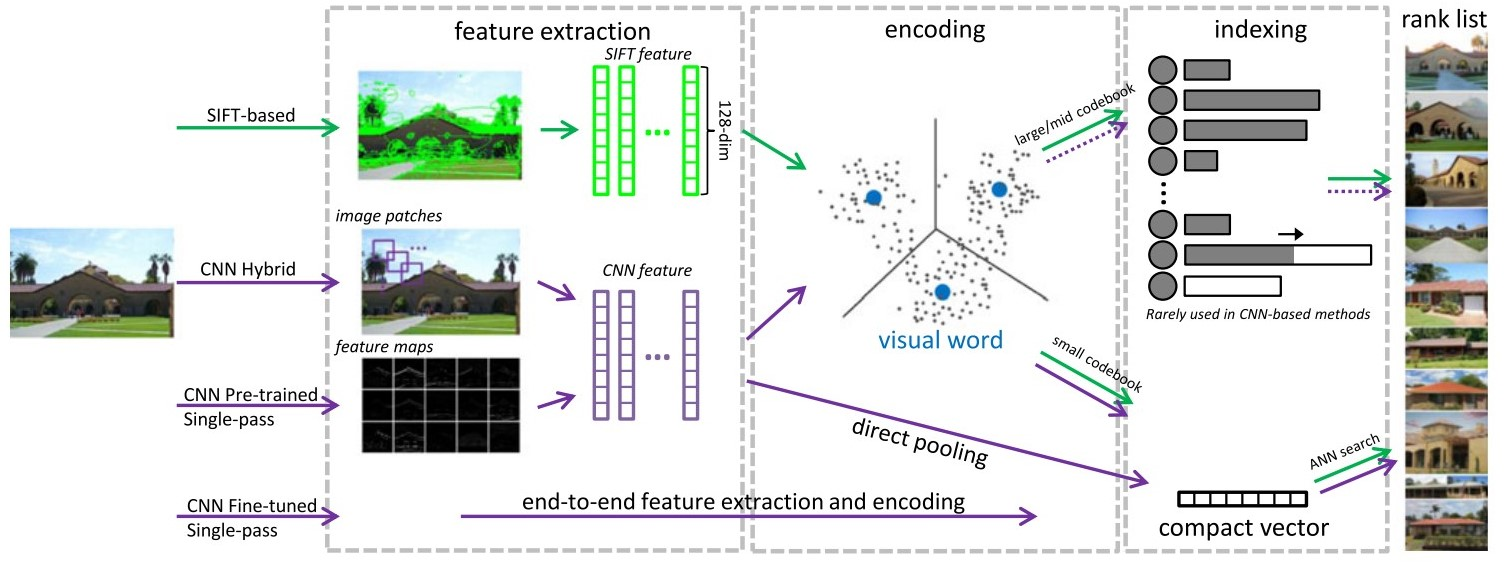
\includegraphics[scale=0.5]{img/img-rec-pipeline.jpg}
    \caption{general instance retrieval pipeline as presented in \cite{}}
\end{figure}

For SIFT based recognition we tried multiple feature extractors such as SIFT, RootSIFT and ORB.
Encoding used was VLAD \cite{} from \cite{}.
For the CNN based recognition we limited ourselves to the Pre-trained CCNs since our dataset was relatively small and unsuitable for finetuning.
The CNN method chosen was R-MAC \cite{} from \cite{}
We had trouble finding suitable CNN feature extractor implementations in python (we found multiple in Matlab) so we were unable to compare multiple approaches.
The search methods tried were Aproximate NN from [pynndescent], Product Quantization (PQ) from [nanopq], Locally Sensitive Hashing (LSH) from [nearpy] and KDTree and BallTree from [sklearn].
In the end we choose BallTree NN search since it outperformed most of the searches in both time needed to create the search structure and time needed for addition of new element to the search
It is also suitable for search in high-dimensional spaces. 

The core of the pipeline consists of SIFT feature extractor, VLAD encoding and BallTree search.
For preprocessing we scale large images to maximum width of 640px while preserving the aspect ratio.
We convert images to grey-scale and apply Contrast Limited Adaptive Histogram Equalization (CLAHE) \cite{} to increase the number of features extracted in low-light environments. 
For post processing we compare a number of matching features between the inputted and retrieved images.
If number of matching features is less then 16 we discard the retrieved image and determine that no matching coaster was found in the image. 
We also tried and discarded geometric feature matching with RANSAC \cite{} but this greatly increased the processing time needed and usually only let to less then 4 feature matches between the images.


\subsection{Finder\&Matcher Integration}

We first input the image into the Finder, as output we receive a list of bounding boxes.
If the list is empty we input an unaltered image to the matcher.
Otherwise we do for each bounding box separably the following: 
we extract part of the image inside the bounding box, 
stretch the cropped image to a square - this helps with feature extraction since most coasters are of square-ish shape - 
and input the stretched image into the Matcher.
As the output we have a list of best matched coasters for each bounding box or the whole image. 



\section{Results}
% - Interpretation of the results. 
% - How do your results compare to the prior work?
% - How do they meet the needs of your application?
Our application is in very specific field, as such we had to create our own dataset for training and testing.
We tested the Finder and Matcher independently and as a unified system.
The relevant metrics for finder were recall and precision. For Matcher we opted for accuracy since there are 100+ instances present.

\subsection{Dataset}
% dataset creation and other stuff
In making a coaster finder dataset we lacked coasters due to coaster scarcity in Iceland where this project was worked on.
To solve this issue the images of coasters were printed on paper to create the percieved appearance of a coaster. The images of coasters
were found on a coaster collection database found on the website coasters.eu \cite{}. The printed images were cut out and roughly sized proportionally to real coasters. 
These cutouts were placed in various locations within the authors reach and photographed. The total number of coaster cutouts for the 
training dataset was 120 with some additional photos taken per coaster and 5 empty photos. This provides a dataset of 184 but 2 photos
including faces and 4 photos including beer in a glass were included later upon retraining to increase environment specific learning.
Heavy augmentation was also used to bring the total image count to 498 images. List of used augments is Flip, 90°Rotate, Crop, Shear, Grayscale, Hue, Brightness, Exposure, Blur,
Bounding Box: Rotation, Bounding Box: Shear, Bounding Box: Brightness, Bounding Box: Noise. The augments were applied randomly and automatically using roboflow.

\newpage

\subsection{Finder}

To experiment with the finder results a new test dataset was created. The new dataset had 44 images with 50 coasters and various other objects located
within certain images. Two models were tested, both were fine tuned on yolov5s. One had 184 images, specifically missing the two images containing faces and four images containing beer.
The second model did contain the previously missing images and was heavily augmented. The results are as follows: 

\begin{table}[H]
    \centering
    \begin{tabular}{ c|c c c } 
     version & recall & precision & avg conf. \\ \hline
     Synthetic & 0.96 & 0.83 & 0.74 \\ 
     Augmented & 0.9 & 0.85 &  0.78 \\ 
    \end{tabular}
    \caption{Finder results}
\end{table}
% Synthetic version:
%     Recall = 0.96, Precision = 0.83
%     Average confidence of correct detections = 0.74
% Augmented version:
%     Recall = 0.9, Precision = 0.85
%     Average confidence of correct detections = 0.78

\subsection{Matcher}

The testing of different feature extractors was done on the Synthetic dataset with VLAD encoder and BallTree search.
Unfortunately we don't have numerical results for different search methods however while implementing them it was clearly apparent that BallTree and KDTree outperformed all other methods in time needed to retrieve, add and initialize the items.

\begin{table}[H]
    \centering
    \begin{tabular}{ c|c c  } 
    features & accuracy & FPS \\ \hline \hline
    SIFT     & 0.78     & 1.5 \\ 
    RootSift & 0.75     & 1.4 \\ 
    ORB      & 0.38     & 9.1 \\
    R-MAC    & 0.04     & 0.7 \\ \hline
    SIFT+Finder & 0.96 & 1.48 \\
    \end{tabular}
    \caption{Matcher feature extractor results}
\end{table}

\subsection{Finder\&Matcher}

The testing of fully integrated system was done on the testing dataset of 44 images, same as testing if the Finder.
The accuracy achieved with the Finder model trained on the Synthetic dataset was \textbf{0.94}.

\section{Discussion}

The comparison of the features used by Matcher, the basic SIFT outperformed RootSIFT which go against the general consensus on the feature extractors.
We have no explanation of the poor results of R-MAC other than incorrect implementation on our side, since general consensus on R-MAC is that it outperforms standard SIFT based features.

As we can see from the results of the Finder, the training on the Augmented dataset reduced recall and improved precision.
This behavior might be undesirable in the integrated system since it is better for the Matcher to focus on false positive area rather than to miss the coaster in the scene entirely. To improve the recall of the finder the training data set needs to be expanded to a more coaster like environment to train the model on background objects. Augmentation use would need to be toned down if it were to be used at all.
The combination of both systems leads to the best results, it allows the Matcher to focus only in potentially interesting areas, as we can se in fig2 where the addition of the Finder narrows area of interest thus decreasing total number of features in the image and prevents matcher from finding an incorrect coaster.

\begin{figure}[H]
    \center
    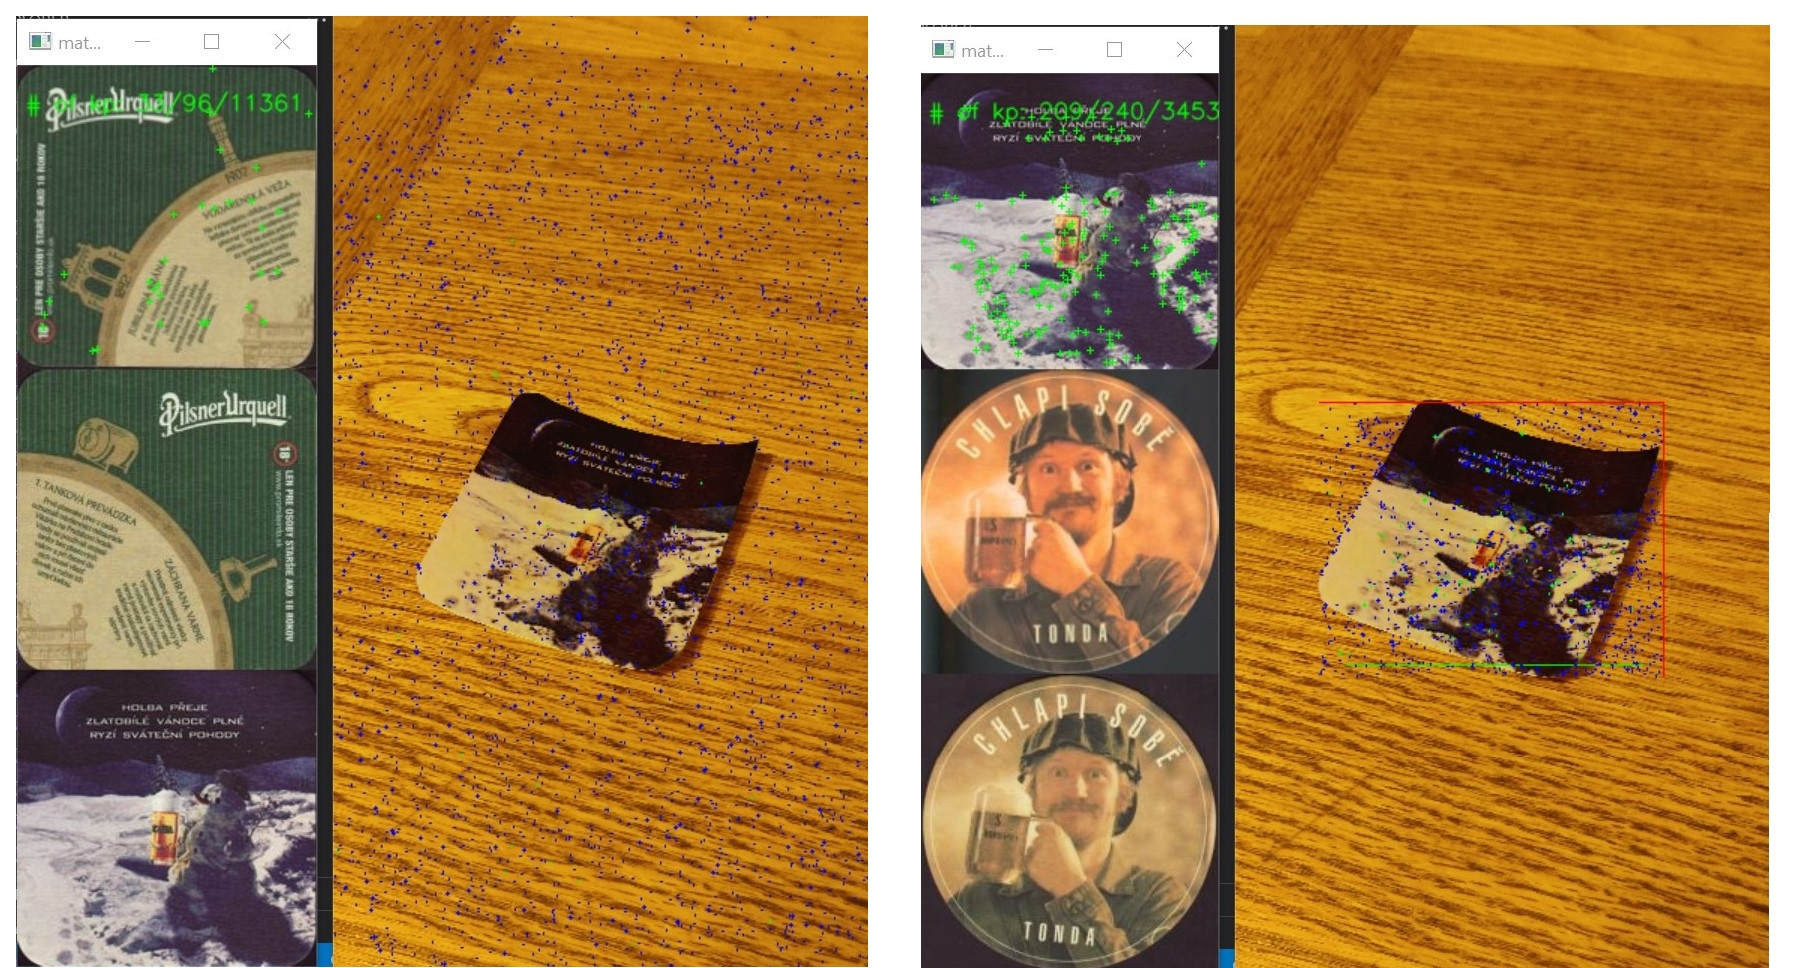
\includegraphics[scale=0.4]{img/addedFinder.jpg}
    \caption{only Matcher (left), Matcher\&Finder (right)}
\end{figure}

In section 3.3 we also included results of SIFT features combined with the Finder. The use of Finder on the Synthetic dataset are not representative of Finders general performance since it was trained on this dataset.
However we might view these as idealized results if the Finder finds the coaster in the image 100\% of the time.


\section{Conclusion}
% - Conclusions and future work
% - What does your work tell you about the technical feasibility of achieving your goals?
% - Ideas for future work on the project or spin-offs.





% \begin{figure}[htbp]
%     \center
%     \includegraphics[scale=0.06]{img/photo.jpg}
%     \caption{Sydney, NSW}
% \end{figure}

\newpage

% ------------------------------------------------------------------------------
% Reference and Cited Works
% ------------------------------------------------------------------------------

\bibliographystyle{IEEEtran}
\bibliography{References.bib}

% ------------------------------------------------------------------------------

\end{document}